\documentclass[12pt, a4paper, oneside]{book}


%------------------------
% IMPORT PACKAGES
%-----------------------
%\usepackage{amsthm}

%\usepackage{mathtools}
%\usepackage{algpseudocode}
%\usepackage[chapter]{algorithm}
\usepackage{amssymb}
\usepackage{amsmath}
%\usepackage{graphicx}

%\usepackage{caption}
%\usepackage{fancyvrb}
\usepackage{array}
\usepackage[nonumberlist, acronym]{glossaries}
%\usepackage{hyperref}
\usepackage{epigraph}
\usepackage{url}
%\def\UrlBreaks{\do\/\do-}
\usepackage{breakurl}
\usepackage[breaklinks]{hyperref}
%\expandafter\def\expandafter\UrlBreaks\expandafter{\UrlBreaks%  save the current one
%	\do\a\do\b\do\c\do\d\do\e\do\f\do\g\do\h\do\i\do\j%
%	\do\k\do\l\do\m\do\n\do\o\do\p\do\q\do\r\do\s\do\t%
%	\do\u\do\v\do\w\do\x\do\y\do\z\do\A\do\B\do\C\do\D%
%	\do\E\do\F\do\G\do\H\do\I\do\J\do\K\do\L\do\M\do\N%
%	\do\O\do\P\do\Q\do\R\do\S\do\T\do\U\do\V\do\W\do\X%
%	\do\Y\do\Z}
\usepackage{listings}
\usepackage{systeme}
\usepackage{cancel}
\usepackage{color}
\usepackage[table, dvipsnames]{xcolor}
\usepackage{tikz}
\usepackage{subcaption}
\usepackage{dsfont}

\usepackage{booktabs}
\usepackage{makebox}
\usepackage{tabularx}
\usepackage{blindtext}

\usepackage{colortbl}
\usepackage{xcolor}
\usepackage{rotating}

\usepackage{array}
\usepackage{lipsum}

\usepackage{natbib}


\usepackage{IEEEtrantools}

\usepackage{cleveref}





\DeclareMathOperator*{\argmax}{arg\,max}
\DeclareMathOperator*{\argmin}{arg\,min}

%% remark theoremstyle
%\newtheoremstyle{break}
%{\topsep}{\topsep}%
%{\itshape}{}%
%{\bfseries}{}%
%{\newline}{}%
%\theoremstyle{break}
%\newtheorem{remark}{Remark}[section]

% problem theoremstyle
%\newtheoremstyle{problemstyle}  % <name>
%{10pt}  % <space acbove>
%{10pt}  % <space below>
%{\normalfont} % <body font>
%{}  % <indent amount}
%{\bfseries\itshape} % <theorem head font>
%{\normalfont\bfseries:} % <punctuation after theorem head>
%{.5em} % <space after theorem head>
%{} % <theorem head spec (can be left empty, meaning `normal')>
%\theoremstyle{problemstyle}
%\newtheorem{problem}{Problem}[section] % Comment out [section] toremove section number dependence
%\newtheorem{definition}{Definition}[section]
%\newtheorem{theorem}{Theorem}[section]
%\newtheorem{proposition}{Proposition}[section]
%\newtheorem{remark}{Remark}[section]
%\newtheorem{lemma}{Lemma}[section]
% create command for variance in math mode
%\newcommand{\Var}[1]{\operatorname{Var}\left[#1\right]}
%\newtheorem{thm}{Theorem}[section]
%\newtheorem{mydef}{Definition}[section]
%\newtheorem{myexample}{Example}[section]
%\newtheorem{myprop}{Proposition}[section]

%\newcommand{\source}[1]{\caption*{Source: {#1}} }

%\renewcommand\textflush{flushright}
\setlength\epigraphwidth{.6\textwidth}


\newacronym{i.i.d}{i.i.d}{Independent and identically distributed}
\newacronym{RCLL}{RCLL}{Right continuous with left limit}
\newacronym{SV}{SV}{Stochastic Volatility}
\newacronym{JD}{JD}{Jump Diffusion}
\newacronym{GBM}{GBM}{Geometric Brownian Motion}
\newacronym{PDE}{PDE}{Partial Differential Equation}
\newacronym{MPT}{MPT}{Modern Portfolio Theory}
\newacronym{chf}{chf}{characteristic function}
\newacronym{pdf}{pdf}{probability density function}
\newacronym{FFT}{FFT}{Fast Fourier Transform}
\newacronym{DE}{DE}{Differential Evolution}

\makeglossaries


\definecolor{dkgreen}{rgb}{0,0.6,0}
\definecolor{gray}{rgb}{0.5,0.5,0.5}
\definecolor{mauve}{rgb}{0.58,0,0.82}

\lstdefinestyle{mystyle}{
	backgroundcolor=\color{gray!30},   
	commentstyle=\color{green},
	keywordstyle=\color{blue},
	numberstyle=\tiny\color{gray},
	stringstyle=\color{black},
	basicstyle=\footnotesize,
	breakatwhitespace=false,         
	breaklines=true,                 
	captionpos=b,                    
	keepspaces=true,                 
	numbers=left,                    
	numbersep=5pt,                  
	showspaces=false,                
	showstringspaces=false,
	showtabs=false,                  
	tabsize=2
}

\lstset{style=mystyle}

\begin{document}

%----------------------------------------------------------------------------------------
% COVER PAGE
%----------------------------------------------------------------------------------------
\pagestyle{empty}
\begin{titlepage}
	\begin{center}
		\normalsize 
			\textsc{Politecnico di Milano}\\
			School of Industrial and Information Engineering\\
			Master of Science in Mathematical Engineering\\

	\end{center}
	\vspace{.6cm}
	
	\begin{figure}[htpb]
		\centering
		
\includegraphics[width=4cm]{Cover/polimi.eps} %
	\end{figure}
	\vspace{.6cm}
	
	\begin{center}
		\LARGE
			\textsc{CRYPTOASSETS IN ASSET ALLOCATION:}
	\end{center}
	\begin{center}
	    \fontsize{16}{11}\textsc{a new Asset Class}
	\end{center}
	\vspace{1.6cm}

	\begin{flushleft}
		\large
		\begin{tabular}{ll}
		Supervisor: & Prof.	Daniele Marazzina \\
		& Prof. Ferdinando M. Ametrano
		\end{tabular}
		\vspace{1cm}
	\end{flushleft}
	
	\begin{flushright}
		\large
		Master thesis by:
		Matteo Avigni\\
		ID: 883093\\		
	\end{flushright}
	
	\vspace*{\fill}
	\begin{center}
		Academic year 2018-2019
	\end{center}
	
\end{titlepage}


%----------------------------------------------------------------------------------------
% ABSTRACT
%---------------------------------------------------------------------------------------

%% Set page numbers of the introduction to roman  
\frontmatter
\pagestyle{plain}
%\chapter{Abstract}
\label{chpr:abstract}

aaaaaaaaa

%\cleardoublepage
%\vspace*{\fill}
%\epigraph{\textit{The secret to happiness is freedom. \\ And the secret to freedom is courage.}}{Thucydides}
%\vspace*{\fill}


%----------------------------------------------------------------------------------------
%	LIST OF CONTENTS/FIGURES/TABLES PAGES
%----------------------------------------------------------------------------------------

\tableofcontents
\listoftables
\addcontentsline{toc}{chapter}{List of Tables}
\listoffigures
\addcontentsline{toc}{chapter}{List of Figures}


\glsaddall
\printglossaries

\chapter{Abstract}
\label{chpr:abstract}

aaaaaaaaa
%\chapter{Acknowledgements}
\label{chpr:acknowledgement}

***add acknowledgements***

\bigskip
\noindent

\bigskip 
\noindent
aaaaaaa


%----------------------------------------------------------------------------------------
%	THESIS CONTENT - CHAPTERS
%----------------------------------------------------------------------------------------

\mainmatter

\chapter{Introduction}
\label{chpr:intro}
\bigskip

Cryptoassets are a type of private asset that depend primarily on cryptography and distributed ledger technology as part of their perceived or inherent value. Since the launch of Bitcoin on the $3^{rd}$ of January 2009 a wide range of cryptoassets have been established, each one with slightly different characteristics.

\bigskip
Although the number of existing cryptoassets is vast, the biggest share of market in terms of capitalization and exchanged volumes is detained by only few of them. In the  \textit{Crypto Index} \citep{cryptoindex} daily exchanged volumes have been collected for 12 major cryptoassets from several exchanges. The collection of data has considered only the crytoassets which satisfy some consistencty criteria. Using this dataset one can plot the 1-month rolling average of the percentage of exchanged volumes for each of them, where 100\% is the sum of the volume exchanged for all of them. This configuration is shown in figure \ref{introfigure}: the black line represents the sum of the percentage of Bitcoin, Ethereum, Ripple and Litecoin. This line lies always above 90\%. This implies that, in the period between January 2016 and May 2019, considering those cryptoassets allows the analysis produced in this thesis to cover at least the 90\% of the market.


\begin{figure}[H]
		\centering
		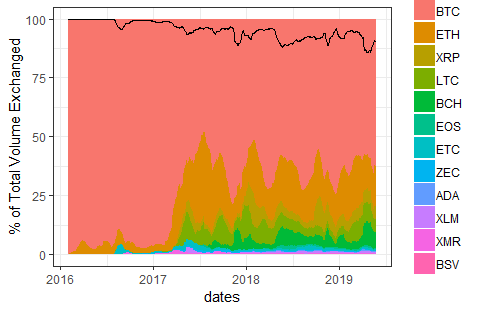
\includegraphics[width=12.5cm]{Images/tot_volumi.png} %
        \caption{1-month rolling average percentage of exchanged volumes by cryptoasset}
        \label{introfigure}
\end{figure}

Bitcoin, Ethereum, Ripple and Litecoin are, therefore, the cryptoassets this thesis is focusing on and below are rapresented their characteristics, similarities and differences.
\bigskip

Bitcoin (BTC) was presented in \citep{BTC2008} as a peer-to-peer protocol for electronic cash that would allow online payments to be sent directly from one party to another without going through a financial institution. Initially it was only used by a niche of people in online cryptology forums to experiment with the transaction protocol. It took a few years for Bitcoin to gain public notoriety, while the price kept rising and having quick crashes.
In particular, Bitcoin generated a lot of buzz in 2017, a year that registered the price increase from 998\$ to 13,412\$ in January 2018 with an all-time high of 19,666\$ on the $17^{th}$ of December. As usually seen during any of the history's gold rushes, many people joined the trend and tried to jump on the train of quick and easy money and were let down when the price collapsed to a level of six thousand dollars in 2018 and has lately stabilized around three thousands.
Recently there has been again more and more talks about Bitcoin and cryptoassets in general due to a group of important payment firms that, together with Facebook, have announced a project of a new global cryptocurrency: Libra. Setting aside the mere numerical value of the price, Bitcoin was the first protocol to solve the problem of double-spending without the need for a centralized party: bitcoins can be transferred but not duplicated, as they only exist as validated transactions in the distributed blockchain. In the same way that e-mail substituted post mail, Wikipedia and other knowledge-based website outdated paper encyclopedias, music and film streaming services are becoming the new user friendly experience for the two industries, Bitcoin presents itself as a system to exchange wealth between users without the need for banks or other trusted third parties.
Furthermore, Bitcoin is the first digital currency to achieve scarcity in the digital realm: its monetary policy based on deterministic supply, mimics the progressive scarcity of gold. It is this deterministic supply that make Bitcoin a suitable long-term investment, since it prevents arbitrary increase in its total available amount, unlike what happens with fiat money.
For these reasons I believe that Bitcoin can be digital gold with an embedded secure network and its characteristics make it resemble more closely to a cryptoasset rather than a cryptocurrency. Even though there are a number of supporters of this idea, for instance in \citep{digitalgold} it is shown that Bitcoin possesses the same hedging abilities of gold, there is yet no general consensus on the matter and different studies get to the opposite result: see for example \citep{klein}.
Bitcoin has been called many names: a bubble, a Ponzi scheme, but also defined as sound money and store of value. I agree with the latter and believe that if Bitcoin is true digital gold, then its value will express the huge potential that has been so far limited by scepticism and misunderstandings.

\bigskip
Ethereum (ETH) is the name of a blockchain company that has created the digital token ether. But Ethereum and ether are now used interchangeably to refer to the cryptocurrency.
Ether is backed by a blockchain, much like bitcoin, but the technology is slightly different and aimed at a specific use case: smart contracts.
The cryptocurrency ether is required by developers who want to build \textit{apps} on the Ethereum blockchain and by users who want access to interact with the smart contracts on the platform.

\bigskip
Ripple (XRP) markets itself as a cross-border payments solution for large financial institutions based on blockchain technology.
At the moment, an international payment may take a few days to be made with a very high cost. A challenge for banks is high-volume, but low-value, transactions.
These can often be expensive and unprofitable for banks because it takes a lot of effort to move the money and the percentage cut won’t be as high as for a larger transaction.
Ripple is trying to solve this problem via its technology.
The Ripple digital currency, known as XRP, can be used by enterprise to get instant liquidity needed in a high-value transaction, without having to pay fees.
XRP acts as a bridge between fiat currencies during a transaction. Ripple said transactions in XRP can be settled in four seconds, faster than any major cryptocurrency right now.

\bigskip
Litecoin (LTC) is probably bitcoin’s closest rival in terms of the use case. Founder Charlie Lee has, on numerous occasions, said that this cryptocurrency can be used for payments because it’s faster than bitcoin.
Litecoin transactions take just over two minutes to go through, compared to an average of around nearly 300 minutes for bitcoin.
There is a limited supply of 84 million litecoins, compared to 21 million bitcoins.

\bigskip
This work intends to study the correlation between the crypto-world, represented by the four major cryptoassets in terms of market capitalization, and other types of standard assets. In particular, I tried to understand if there is significant difference among these four cryptoassets in terms of correlation with the market.
Then, diversification property of cryptoassets added to a portfolio is explored by computing the optimal allocation for different levels of risk and expected return in a Markowitz mean-variance framework.

\bigskip
In literature there are several papers about the inclusion of Bitcoin in an investment portfolio, for example \citep{bouri} where the authors arrive to the conclusion that Bitcoin acts well in terms of diversification, less as a hedge or safe haven.
In \citep{weiyi} the authors analysed a portfolio composed only by ten major cryptoassets and found out that diversifying between crypto yield higher returns with lower risk with respect to single cryptoassets. 
Then in \citep{corbet} the authors analysed the role of btc, ltc and xrp in an investment portfolio with other indexes. It turned out that cryptoassets can be considered as a new investment asset class since they are interconnected with each other and have similar patterns of connectedness with other asset classes.



\bigskip
\noindent
The present thesis has been written during the author's collaboration with the Digital Gold Institute (\href{https://www.dgi.io/}{https://www.dgi.io/}), a research and development center focused on teaching, consulting and advising about scarcity in the digital domain (Bitcoin and cryptoassets) and the underlying blockchain technology.


\section{Thesis structure}
\bigskip
This work is structured into 6 chapters.

\noindent
Chapter \ref{chpr:ch2} presents the state of the art in cryptoassets usage for diversification in asset allocation.

\noindent
In chapter \ref{chpr:ch3} a study on the empirical correlation between the assets taken into considerations is done. Here is also checked the significance of each correlation value by performing two statistical tests, Pearson's t-test and a permutation test. Finally, there's a deeper analysis of correlations between cryptoassets, which is done by investigating the rolling correlations and their significance.

\noindent
In chapter \ref{chpr:ch4} some consideration about cryptoassets returns are done.

\noindent
Chapter \ref{chpr:ch5} analyses the optimal allocation of a portfolio composed of cryptoassets and “classic” instruments

\noindent
Chapter 6 concludes this work and sums up the main results. It also includes some final remarks to this study.



\section{Dataset  Presentation}
\bigskip
The dataset on which we focus our study contains 886 observations of the prices of 19 assets valued daily (excluding holidays and weekends) from the $1^{st}$ of January 2016 till the $24^{th}$ of May 2019 (some data provided by Bloomberg and others, the ones related to the cryptoassets, by Coinmarketcap).
The assets we included in our analysis are grouped into five different classes, as explained in the following list (in brackets we indicate the shortened name that is used in the tables and graphs):
\begin{enumerate}
    \item Cryptoassets:
    \begin{itemize}
        \item Bitcoin (btc): Value of a single bitcoin, quoted in dollars.
        \item Ethereum (eth): Value of a single ether, quoted in dollars.
        \item Litecoin (ltc): Value of a single litecoin, quoted in dollars.
        \item Ripple (xrp): Value of a single ripple, quoted in dollars.
    \end{itemize}
    \item Stock Indexes:
    \begin{itemize}
        \item S\&P500 (sp500): American stock market index based on 500 large company with stock listed either on the NYSE or NASDAQ.
        \item EURO STOXX 50 (eurostoxx): equity index of eurozone stocks, covering 50 stocks from 11 eurozone countries.
        \item MSCI BRIC (bric): market cap weighted index designed to measure the equity market performance across the emerging country indexes of Brazil, Russia, India and China.
        \item NASDAQ (nasdaq): market cap weighted index including all NASDAQ tiers (Global Select, Global Market and Capital Market).
    \end{itemize}
    \item Bond Indexes:
    \begin{itemize}
        \item BBG Pan European (bond europe): Bloomberg Barclays Pan European Aggregate Index that tracks fixed-rate, investment-grade securities issued in different European currencies.
        \item BBG Pan US (bond us): Bloomberg Barclays US Aggregate Bond Index, a benchmark that measures investment grade, US dollardenominated, fixed-rate taxable bond market.
        \item BBG Pan EurAgg (bond eur): similar to the Pan European but it only considers securities issued in Euros.
    \end{itemize}
    \item Currenncies
    \begin{itemize}
        \item EUR/USD (eur): spot value of one Euro in US dollars.
        \item GBP/USD (gbp): spot value of one British Pound in US dollars.
        \item CHF/USD (chf): spot value of one Swiss Franc in US dollars.
        \item JPY/USD (jpy): spot value of one Japanese Yen in US dollars.
    \end{itemize}
    \item Commodities:
    \begin{itemize}
        \item Gold (gold): price of gold measured in USD/Oz.
        \item WTI (wti): price of crude oil used as benchmark in oil pricing and as the underlying commodity in the NYMEX oil future contracts.
        \item Grain (grain): S\&P GPSCI index that measures the performance of the grain commodity market.
        \item Metals (metal): S\&P GSCI Industrial Metals index that measures the movements of industrial metal prices including aluminium, copper, zinc, nickel and lead.
    \end{itemize}
\end{enumerate}


\chapter{Conclusions}
\label{chpr:conclusion}

\bigskip
aaaaaaaaaa


%----------------------------------------------------------------------------------------
%	THESIS CONTENT - APPENDICES
%----------------------------------------------------------------------------------------
\bibliographystyle{apalike}
\bibliography{Bibliography/my_bibliography}

\appendix
\chapter{Title }
\label{app:A}

aaaaaaaaaa



\backmatter
%----------------------------------------------------------------------------------------
%	BIBLIOGRAPHY
%----------------------------------------------------------------------------------------

\backmatter
%\nocite{*}




\end{document}  